\chapter{Umsetzung}
Im Rahmen dieser Arbeit entstand ein in C++ geschriebenes Programm welches den Marching Cubes Algorithmus auf eine Voxelmenge anwendet und das Resultat via OpgenGL visualisiert. Des Weiteren ist es möglich das verarbeitete Model als STereoLithography (.stl) Datei zu exportieren.
\section{Marching Cubes}
\label{sec:mcUms}
Der Marching Cubes Algorithmus ist das Herzstück der entstandenen Applikation er ermöglicht die Umrechnung der gegebenen Voxel Datenmenge in eine polygonale Darstellung welche sich im später vergleichsweise einfach darstellen lässt.
\subsection{Allgemein}
Die Implementierung ist eine angepasst Version der von [ref] bereitgestellten Umsetzung. Die wesentlichen Änderungen sind die Auslagerung der Funktionen in eine eigenen Klasse und das verwenden anderer Datenstrukturen. Durch die Umstellung auf STL-Behälter und der daraus folgende Verzicht auf C-Strukturen welche zur Laufzeit immer neuen Speicher anfordern konnte die Geschwindigkeit enorm erhöht werde.
\subsection{Schnittstelle (Klasse)}
\begin{figure}[H]
	\centering
	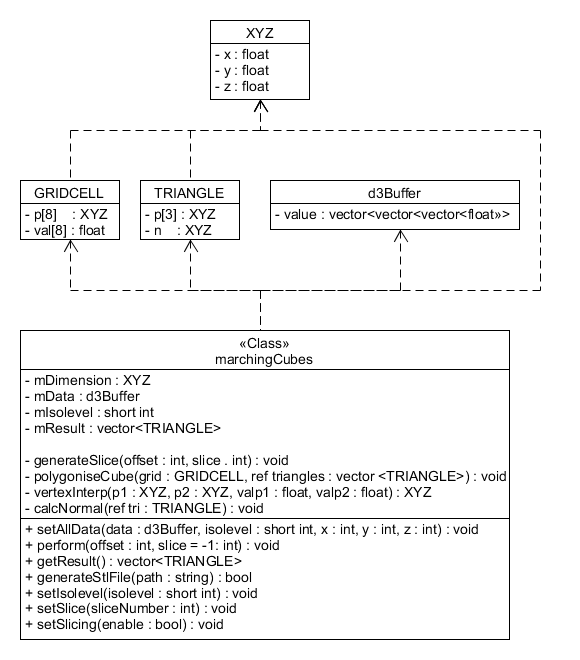
\includegraphics[width=.90\textwidth]{marchingCubes}
	\caption{UML-Diagramm der marchingCubes Klasse}
	\label{fig:marchingCubes}
\end{figure}

\subsubsection{Datentypen}
Neben den üblichen Datentypen wurden zur Vereinfachung komplexere Strukturen verwendet.\\
\begin{itemize}
	\item \textbf{XYZ} beschreibt einen Punkt im dreidimensionalen Raum.
	\item \textbf{GRIDCELL} ist die Repräsentation eines Voxel-Würfels. 
	\item \textbf{TRIANGLE} Repräsentiert ein Dreieck mithilfe seiner drei Eckpunkte und seiner Normalen.
	\item \textbf{3dBuffer} bildet ein Voxelgitter als dreidimensionalen Vektor im Speicher ab.
\end{itemize}

\subsubsection{Funktionen}
Um ein grundlegendes Verständnis zu bieten werden hier die öffentlichen Methoden der Klasse kurz beschrieben. 
\begin{itemize}
	\item \textbf{setAllData:} Da während der Laufzeit des Programmes nur eine Instanz der marchingCubes-Klasse instanziiert wird, ist es notwendig diese, wenn nötig, mit neuen Werten zu initialisieren. Es wird das gesamte Voxelgitter (data) sowie der zu verwendende Schwellwert (isolevel) für die Berechnung mitgegeben.
	\item \textbf{perform:} Diese Funktion führt den Marching Cubes Algorithmus auf dem zuvor via setAllData gesetzten Voxelgitter aus. Es bestehen zwei Möglichkeiten des Aufrufs. Zum Einen mit beiden Parameter und zum Anderen mit nur dem ersten (offset) Parameter. Bei der ersten Variante wird nur eine Scheibe des Voxelgitters betrachtet, wobei der erste Parameter die Dicke der Scheibe und der zweite die Position der Scheibe im Gitter kennzeichnet. Bei der zweiten Variante wird der gesamte Input betrachtet wobei Parameter ''offset'' die Schrittweite pro Würfel angibt. 
	\item \textbf{getResult:} Hier kann nach dem durchlaufen von perform das Ergebnis des Algorithmus abgegriffen werden. 
	\item \textbf{setIsolevel:} Hier kann der Schwellwert der Voxeln für den Algorithmus nachträglich verändert werden.
	\item \textbf{generateStl:} Das ausführen dieser Funktion persistiert das Ergebnis des Marching Cubes Algorithmus als .stl Datei.
\end{itemize}
\subsection{Verwendung}
Im Programm \ref{prog:MCVerw} ist die Verwendung der Klasse exemplarisch dargestellt.
\begin{program}[H]
	\caption{Verwendung der marchingCubes Klasse}
	\label{prog:MCVerw}
	\begin{CCode}
		int main(){
			marchingCubes *mc = new marchingCubes();
			// set the voxelgrid and the treshold
			mc->setAllData(getRawData(), getIsolevel()); 
			// performs the marching cubes algorithmus on the entire voxelgrid
			mc->perform(getOffset()); 		
			// performs the algorithmus on just a slice of the voxelgrid 
			mc->perform(getOffset(), getSlice()); 
			showPolygons(mc->getResult()); 
			delete(mc);
			return 0;	
		}
	\end{CCode}
\end{program}
\section{File Formate}
Wie bereits im Kapitel \ref{sec:DateiEinf} erwähnt wurden für die Umsetzung die Dateiformate von Analyze 7.5 (.img und .hdr) sowie das STereoLithography (.stl) Format verwendet.
\subsection{Allgemein}
Um eine unnötige Komplexität zu vermeiden wurden für die Analyze-Formate nur lesender und für das STereoLithography Format nur schreibende Zugriff implementiert. Hier bieten sich für spätere Erweiterungen viele Möglichkeiten bezüglich Import/Export (auch für weitere Formate). 
\subsection{Image File (.img)}
Um das Image File auszulesen müssen vorher die Dimensionen des Voxelgitters bekannt sein.  Diese Information erhält man aus dem Header File. Sind die Dimensionen bekannt können mithilfe einer dreifach geschachtelten for-Schleife die einzelnen Voxel-Werte in eine entsprechende Datenstruktur (z.B. dreidimensionales Array) ausgelesen werden. In \citep{AnalyzeFormat} ist eine beispielhafte Implementierung gegeben. Diese wurde für den Prototyp angepasst und integriert.
\subsection{Header File (.hdr)}
Diese Datei ist wie bereits in Kapitel \ref{sec:DateiHead} beschrieben aufgebaut. Auch hier ist in \citep{AnalyzeFormat} eine beispielhafte Implementierung gegeben welche für die Verwendung angepasst und erweitert wurde.
\subsection{STereoLithography (.stl)}
In Abbildung \ref{fig:BINARYSTL} ist bereits der binäre Aufbau einer STL-Datei abgebildet. Die Implementierung (Programm \ref{prog:generateSTL}) richtet sich daher genau an diesen formalen Aufbau.
\begin{program}[H]
	\caption{Generierung einer STL-Datei}
	\label{prog:generateSTL}
	\begin{CCode}
		bool fileHandler::CreateStl(std::string path){
			FILE *fptr = NULL;
	
			int sizeResult = mResult.size();
			fprintf(stderr, "Writing triangles ...\n");
			if ((fptr = fopen(path.c_str(), "a+b")) == NULL) {
				fprintf(stderr, "Failed to open output file\n");
				return false;
			}
			char fileHeader[81] = "solid Test Head";
			char bytes[3] = { 0x00, 0x00 };
			fwrite(&fileHeader, sizeof(fileHeader)-1, 1, fptr);
			fwrite(&sizeResult, sizeof(int), 1, fptr);
			for (int i = 0; i < mResult.size(); i++) {
				fwrite(&mResult[i].n, sizeof(float), 3, fptr);
				for (int k = 0; k < 3; k++)  {
					fwrite(&mResult[i].p[k], sizeof(float), 3, fptr);
				}
				fwrite(bytes, 2, 1, fptr);
			}
			fclose(fptr);
			return true;
		}
	\end{CCode}
\end{program}
\subsection{Schnittstelle (Klasse)}
\begin{figure}[H]
	\centering
	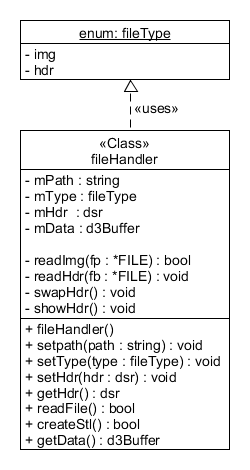
\includegraphics[width=.60\textwidth]{fileHandler}
	\caption{UML-Diagramm der fileHandler Klasse}
	\label{fig:fileHandler}
\end{figure}
\subsubsection{Datentypen}
\begin{itemize}
	\item \textbf{fileType} repräsentiert den zu verarbeitenden Dateityp als Enumeration (img bzw. hdr) 
	\item \textbf{dsr} ist die in Kapitel \ref{sec:DateiHead} beschriebene Repräsentation des Header-Formates als C-Struktur.
	\item \textbf{d3Buffer} wurde bereits im vorhergegangenen Abschnitt (\ref{sec:mcUms}) beschrieben.
\end{itemize}

\section{OpenGL}
\subsection{Allgmein}
\subsection{Schnittstelle (Klasse)}
\begin{figure}[H]
	\centering
	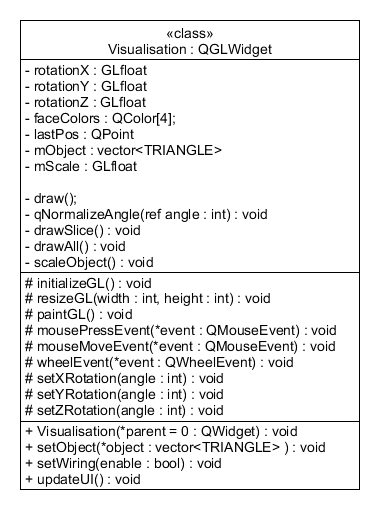
\includegraphics[width=.70\textwidth]{visualisation}
	\caption{UML-Diagramm der Visualisation Klasse}
	\label{fig:visualisation}
\end{figure}

\subsection{Auszüge Implementierung}
\begin{program}
	\caption{Berechnung der Normalen eines Dreiecks}
	\label{prog:calcNormal}
\begin{CCode}
	void marchingCubes::CalcNormal(TRIANGLE &tri){
		XYZ U;
		XYZ V;
		U.x = tri.p[1].x - tri.p[0].x;
		U.y = tri.p[1].y - tri.p[0].y;
		U.z = tri.p[1].z - tri.p[0].z;
		
		V.x = tri.p[2].x - tri.p[0].x;
		V.y = tri.p[2].y - tri.p[0].y;
		V.z = tri.p[2].z - tri.p[0].z;
		
		tri.n[0].x = (U.y * V.z) - (U.z * V.y);
		tri.n[0].y = (U.z * V.x) - (U.x * V.z);
		tri.n[0].z = (U.x * V.y) - (U.y * V.x);
	}
\end{CCode}
\end{program}

\section{Benutzeroberfläche}
\begin{figure}
	\centering
	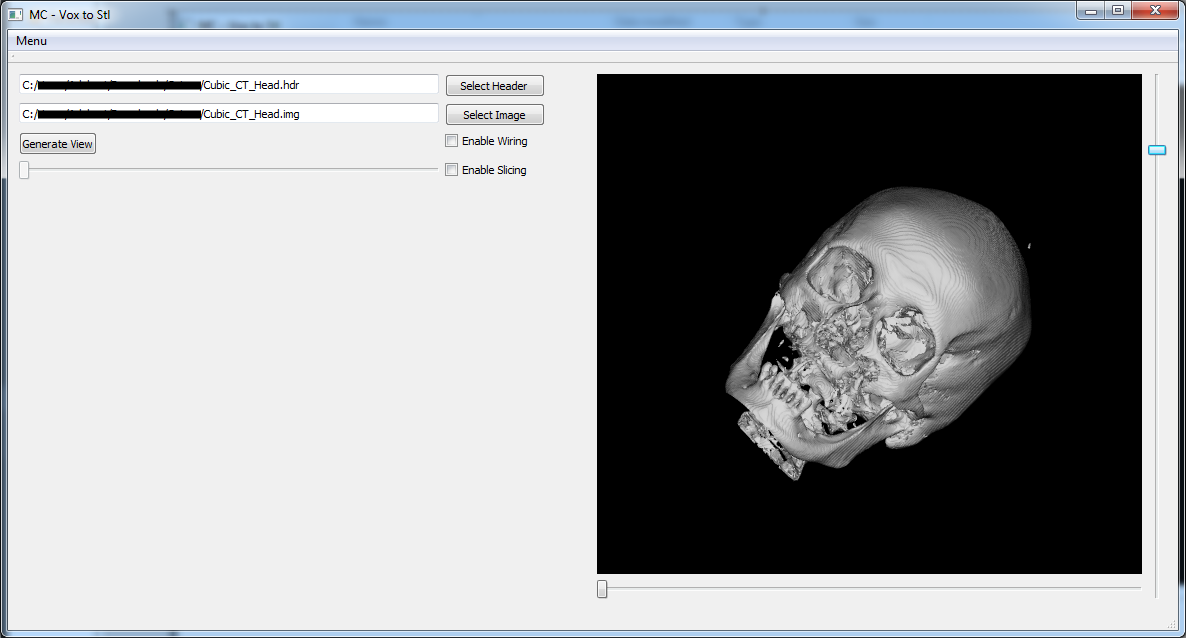
\includegraphics[width=1.0\textwidth]{UI1}
	\caption{Übersicht der Benutzeroberfläche}
	\label{fig:UI1}
\end{figure}

\begin{figure}
	\centering
	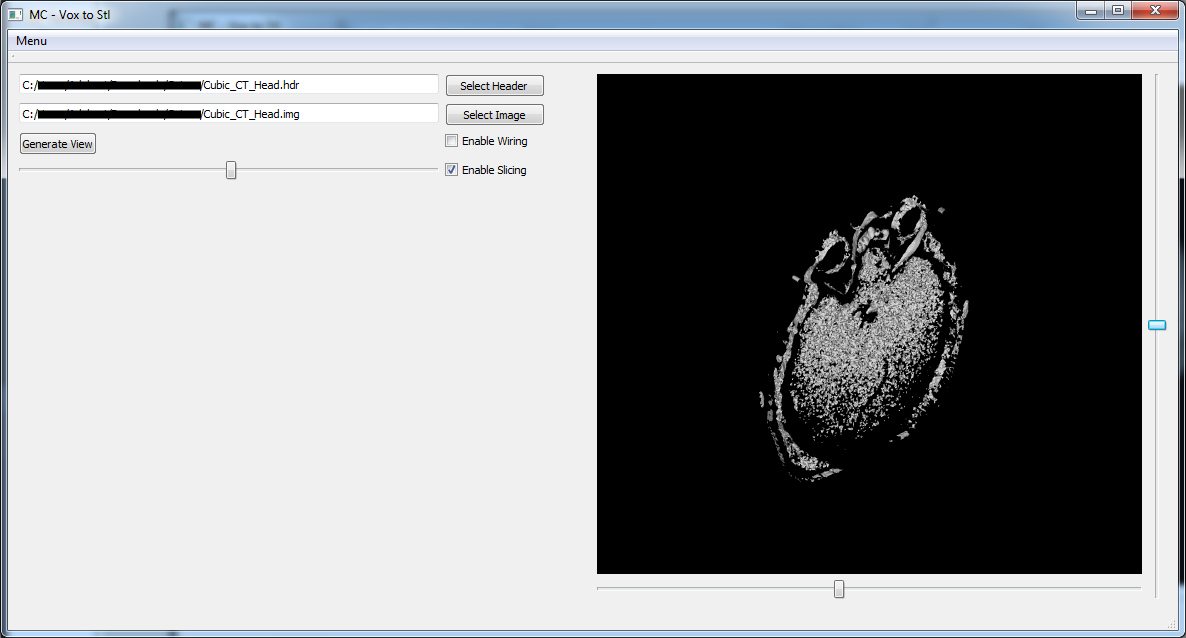
\includegraphics[width=1.0\textwidth]{UISlicing}
	\caption{Programm Slicing aktiviert}
	\label{fig:UISlicing}
\end{figure}

\begin{figure}
	\centering
	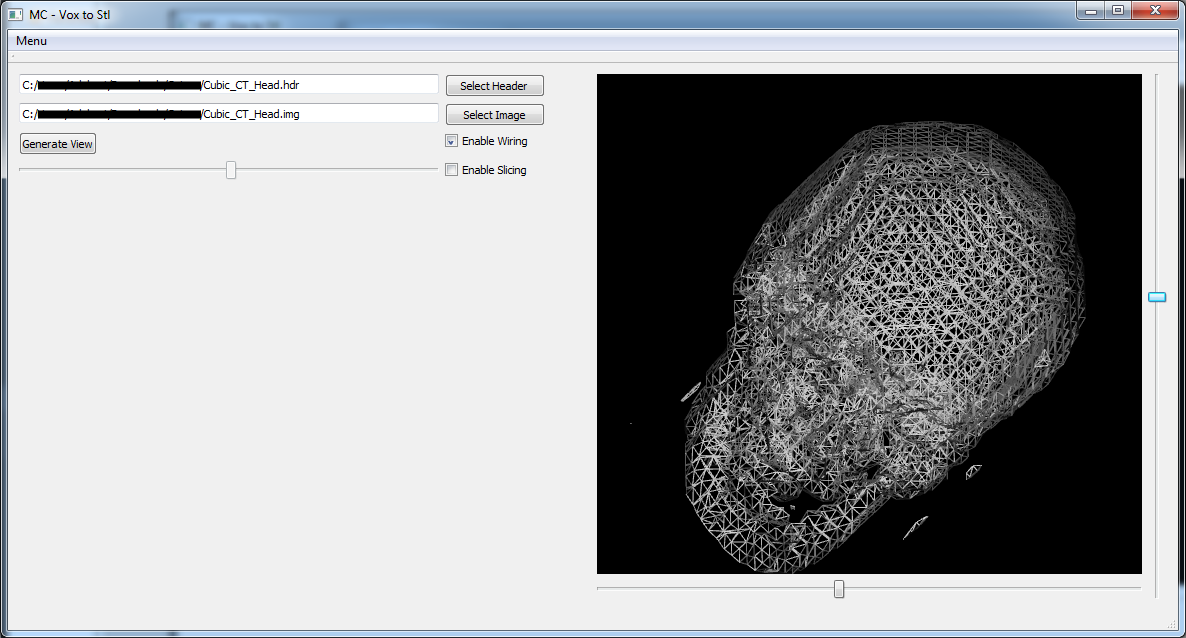
\includegraphics[width=1.0\textwidth]{UIWiring}
	\caption{Programm Wiring aktiviert}
	\label{fig:UIWiring}
\end{figure}